\documentclass[a4paper,10pt]{article}

% ------------------------------------
% packages
\usepackage[a4paper,margin=1in,footnotesep=2.2\baselineskip]{geometry}
\usepackage{multicol}
\usepackage{xcolor}
\usepackage{framed}
\usepackage{emoji}
\usepackage[most]{tcolorbox}
\usepackage{fancyhdr}
\usepackage[tracking=true]{microtype}
\usepackage{ragged2e}
\usepackage{listings}
\usepackage{color}
\usepackage{pagecolor}
\usepackage{pdftexcmds}
\usepackage{geometry}
\usepackage{upgreek}
\usepackage{accents}
\usepackage{caption}
\usepackage{amssymb}
\captionsetup{
  font=small,
  labelfont=bf,
  tableposition=top
}
\captionsetup[figure]{name=\mono{Figure}}

% ------------------------------------
% checksum = SHA-1
\makeatletter
\ifx\pdf@filemdfivesum\undefined\def\pdf@filemdfivesum#{\mdfivesum file}\fi
\let\filesum\pdf@filemdfivesum
\makeatother

% ------------------------------------
% color definitions
\definecolor{armygreen}{rgb}{0.14, 0.71, 0.15}
\definecolor{darkgreen}{rgb}{0.08, 0.48, 0.18}
\definecolor{darkred}{rgb}{0.86, 0.153, 0.153}
\definecolor{azure}{rgb}{0.0, 0.5, 1.0}
\definecolor{bole}{rgb}{0.82, 0.57, 0.22}
\definecolor{dkgreen}{rgb}{0,0.6,0}
\definecolor{gray}{rgb}{0.5,0.5,0.5}
\definecolor{mauve}{rgb}{0.58,0,0.82}
\definecolor{light-gray}{gray}{0.95}
\definecolor{bg}{HTML}{fcfcfa}
\definecolor{bt}{HTML}{ffebe6}

% ------------------------------------
% code styling
\definecolor{shadecolor}{RGB}{180,180,180}
\newcommand{\code}[1]{\colorbox{shadecolor!30}{\mono{#1}}}
\newcommand{\zero}{{$\varnothing$}}
\newcommand{\one}{{$\aleph$}}
\newcommand{\two}{3}
\newcommand{\three}{\uptheta}
\newcommand{\four}{k}
\newcommand{\five}{\raisebox{0.55ex}{\naskh{^^^^062d}}}
\newcommand{\six}{{\hindi{^^^^096d}}}
\newcommand{\seven}{\raisebox{0.3ex}{\robot{^^^^0434}}}
\newcommand{\asserts}{\raisebox{0.10ex}{$\equiv$}}
\colorlet{Gray}{gray!20!}
\tcbset{on line, arc=1pt, leftrule=0.25pt,rightrule=0.25pt,toprule=0.25pt,bottomrule=0.25pt,
	boxsep=3pt, left=0pt,right=0pt,top=0pt,bottom=0pt,
	colframe=white,colback=Gray,  
	highlight math style={enhanced}
}
\lstdefinelanguage{Solidity}{
  %keywords={bool, true, false, return, address, bytes32, bytes4, bytes1, bytes, uint256, uint8, uint, string, if, while, else, case, break},
  keywords={},
  keywordstyle=\color{blue}\bfseries,
  %ndkeywords={function,struct, mapping, export, throw, implements, import, this},
  ndkeywords={},
  ndkeywordstyle=\color{darkgreen}\bfseries,
  identifierstyle=\color{black},
  sensitive=false,
  comment=[l]{//},
  morecomment=[s]{/*}{*/},
  commentstyle=\color{green}\mono,
  stringstyle=\color{orange}\mono,
  morestring=[b]',
  morestring=[b]",
  mathescape=true,
  literate={=>}{${\rightarrow}{}$}{1}
}
\lstset{
  backgroundcolor=\color{light-gray},
  language=Solidity,
  aboveskip=3mm,
  belowskip=3mm,
  showstringspaces=false,
  columns=flexible,
  basicstyle={\footnotesize\mono},
  numbers=none,
  numberstyle=\tiny\color{gray},
  keywordstyle=\color{blue},
  commentstyle=\color{dkgreen},
  stringstyle=\color{mauve},
  breaklines=true,
  breakatwhitespace=true,
  tabsize=3
}

% ------------------------------------
% fonts
\newfontfamily\pro[Path=./]{SFPro.ttf}
\newfontfamily\pbold[Path=./]{SFMonoSemiBold.ttf}
\newfontfamily\mono[Path=./]{SFMono.ttf}
\newfontfamily\mbold[Path=./]{SFMonoSemiBold.ttf}
\newfontfamily\hindi[Path=./]{Martel.ttf}
\newfontfamily\naskh[Path=./]{Naskh.ttf}
\newfontfamily\robot[Path=./]{Roboto.ttf}
\newfontfamily\victr[Path=./]{VictorMono.ttf}

% ------------------------------------
% heading font-size
\usepackage{sectsty}
\usepackage{fontspec}
\sectionfont{\fontsize{12}{15}\selectfont}
\usepackage[utf8]{inputenc}

% ------------------------------------
% footnote positioning
\usepackage[hang,flushmargin,bottom]{footmisc} 

% ------------------------------------
% bibliography
\usepackage[colorlinks=true,
            linkcolor=blue,
            urlcolor=blue,
            citecolor=blue,
            pdfauthor={sshmatrix},
            pdftitle={Helix2 Protocol},
            pdfsubject={Link Service and Protocol},
            pdfkeywords={ethereum, account, abstraction, link, name, decentralised, distributed},
            pdfproducer={sshmatrix},
            pdfcreator={sshmatrix}]{hyperref}
            
% ------------------------------------
% blank footnote
\newcommand\blfootnote[1]{%
	\begingroup
	\renewcommand\thefootnote{}\footnote{#1}%
	\addtocounter{footnote}{-1}%
	\endgroup
}

% ------------------------------------
% header
\pagestyle{fancy}
\fancyhf{}
\lfoot{\footnotesize \mono{\#}\tcbox{\mono{\filesum{\jobname}}}}
\begin{document}
\setcounter{footnote}{0}
\newpage
\topskip15pt

\fancyhead[L]{\footnotesize \mono{author}:\tcbox{\mono{sshmatrix}}}
\fancyhead[R]{{\footnotesize \mono{\href{https://github.com/sshmatrix/research}{github.com/sshmatrix/research/zkTopology}}}}
\fancyhead[C]{{\footnotesize \emoji{dna}}}
\fancyfoot[C]{{\footnotesize \mono{\thepage}}}
\fancyfoot[R]{{\footnotesize \mono{\today} \emoji{dna}}}

\begin{center}
	\textbf{\Large\pbold{\textls[-40]{Topological Interpretation of Elliptic Curves}}}\\
	\vspace{0.075in}
	\textls[-50]{\mono{Topological Interpretation of Finite Cyclic Groups}}\linebreak\linebreak
	\vspace{-0.175in}
	\textls[0]{\mono{Avneet Singh}}\linebreak\linebreak
	\textls[0]{\mono{Interplanetary Company UG}}\linebreak
	\textls[0]{\mono{\href{mailto:sshmatrix@proton.me}{sshmatrix@proton.me}}}\linebreak
\end{center}
\begin{center}
	\textbf{\Large\pbold{ABSTRACT}}\linebreak\linebreak
	\textls[-50]{\mono{Elliptic curves form the backbone of most cryptography today and are expected to feature in the post-quantum world through Zero-Knowlege algorithms. Most literature on Elliptic curves starts from the definition of a cubic symmetric polynomial and builds upon the group theoretic interpretation of finite fields. This may be sufficient to grasp the mere necessary details for implementing Elliptic curves in practise, but not necessarily ideal if one wants to understand why Elliptic curve geometry is unique and useful. To most readers, it can appear that Elliptic curves were drawn from a magic hat. In paper will illustrate that this is clearly not the case and there exists a very legitimate reason for how and why the humanity ended up using Elliptic curves for cryptography.}}
\end{center}
\vspace{0.2in}
\begin{flushleft}
	\textbf{\Large\pbold{INTRODUCTION}}\linebreak\linebreak
	\textls[-50]{\mono{This paper is intended as a standalone appendix to the main paper titled 'Intuitive Interpretation of Non-Interactive Zero-Knowledge Cryptography' [1]. The main paper deals with pretty much the entire field of cryptography starting from basic RSA to advanced Zero-Knowledge algorithms. In interest of conciseness, several important aspects of Elliptic curves couldn't be discussed in detail in the main paper; this document is an attempt to address those shortcomings for the overtly inclined reader. We'll also touch some peripheral topics that have tied number theory and elliptic curves at the hip. Having said that, we'll follow the same theme as the main paper and avoid jargon like plague.\linebreak\linebreak
	}}
	\textbf{\large\pbold{COUNTING STONES}}\linebreak\linebreak
	\textls[-50]{\mono{In order to truly arrive at present day cryptography in a natural sense, we'll start from the very basics of it all. Let's talk about numbers; numbers form the building blocks of cryptography and most mathematics, physics and natural sciences.\linebreak\linebreak 
	}}
	\colorbox{Gray}{\hspace{1mm}\parbox{0.99\textwidth}{\vspace{1mm}\textls[-50]{\mono{To naturally arrive at numbers and their geometry/topology, we will start from a simple yet abstract example of a collection of some stones circa 20,000 BC. Bob's tribe needs stones to make their flint tools and Bob is one of the stone gatherers; this is Bob's story. During this exercise, please refrain from using numbers as you know it in your subconscious. Try to think like Bob, who has no concept of 1, 2, 3 \cdot\cdot\cdot\;etc.\vspace{1mm}}}}}\linebreak\linebreak\linebreak
	\textls[-50]{\mono{Consider a collection of stones that are of {\mbold{approximately}} the same size, shape, weight and texture such that Bob is unable to objectively distinguish any one stone from the rest despite each stone being unique. To quantify this collection of stones into {\mbold{succinct}} information\textsuperscript{\textcolor{blue}{1}}\blfootnote{\textls[-50]{\mono{\textsuperscript{1}{so that Bob can convey information succinctly to others without having to show them the stones}}}} leads Bob into questioning the nature of this collection. In order to {\mbold{differentiate}}/distinguish the stones among each other, Bob does the first natural thing - he names each stone. In other words, he assigns a unique label to each stone (see figure \ref{fig:stones}); such a system is a functioning naming system. Note that there is no condition on actual equivalence among any of the stones, and only an assertion is made that the observer is unable to tell them apart in a describable manner. Using this naming system (\one, \two, \three, \four, \five, {\six\,}, {\seven} as labels), Bob can tell someone else what he saw by showing them the labels, assuming that the labels are an agreed upon standard that everyone recognises. Note that Bob can choose any 'ordering' of the labels and the communication system works the same. This works well for everyone until one day Bob finds a massive pile of stones, all of different shapes and sizes in large quantities. The problem is simply that Bob's naming standard has only a finite number of labels and the stones are too many to each correspond to one label. In other words, Bob has run out of labels. In this moment of tryst, Bob realises that he is not limited by the number of labels at all; he can put two labels together and make a new label! Now he just needs to prescribe a method of deciding which two numbers to put together, how to order them etc.
	}}
\end{flushleft}
\begin{multicols}{2}
	\noindent
	\begin{minipage}{\linewidth}
		\centering
		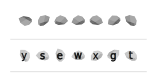
\includegraphics[width=80mm]{./img/Stones.png}
		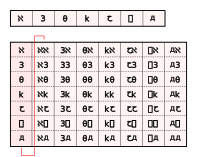
\includegraphics[width=80mm]{./img/Numbers.png}
		\captionof{figure}{\textls[-50]{\mono{Bob's rudimentary number system}}}
		\label{fig:stones}
	\end{minipage}
	\linebreak\linebreak
	\textls[-50]{\mono{To follow Bob's footsteps, we start from {\one} until {\seven}, and then form the next label by joining: the first label with itself (\one\,\one), then first label with second label (\one\,\two), then first label with third label (\one\,\three) and so on until Bob reaches (\one\,\seven). Bob proceeds to do this 'cycling' until he reaches (\seven\,\seven),\linebreak\linebreak
	}}
	\noindent
	\begin{minipage}{\linewidth}
		\centering
		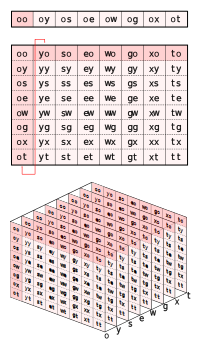
\includegraphics[width=80mm]{./img/Counting.png}
		\captionof{figure}{\textls[-50]{\mono{Symmetric number system after appending {\zero} label}}}
		\label{fig:counting}
	\end{minipage}
\end{multicols}
\begin{flushleft}
	\textls[-50]{\mono{at which point he can describe a lot more stones to his tribe than before. In figure \ref{fig:counting}, we can visualise Bob's naturally constructed number system. Readers by now may have realised that this is exactly like our native {\mbold{natural number}} system with (\one, \two, \three, \four, \five, {\six\,}, {\seven}) {\rightarrow} (1, 2, 3, 4, 5, 6, 7) with no presence of 8, 9 or 0, and it is nothing more. The terminology behind 'natural' is also a lot more intuitive to grasp. We can easily extend this system to count to {\seven\,\seven\,\seven} or {\seven\,\seven\,\seven\,\seven} or {\seven\,\seven\,\seven\,\seven\,\seven}, extending up to any number of digits.\linebreak\linebreak
	}}
	\colorbox{Gray}{\hspace{1mm}\parbox{0.99\textwidth}{\vspace{1mm}\textls[-50]{\mono{In computer science terminology, we know this as base-{\seven} (or base-7) encoding; base-10 is equivalent to the Decimal number system that we commonly use. We can however see that using a very small base quickly leads to overcrowding of digits required to describe any number of stones. On the other hand, a very high base requires keeping a lengthy shared standard among different parties in Bob's ecosystem.\vspace{1mm}}}}}\linebreak\linebreak\linebreak\linebreak
	\textbf{\Large\pbold{DISCOVERING (+, -, {^^^^00d7}, {^^^^00f7})}}\linebreak\linebreak
	\textls[-50]{\mono{In no time, Bob realises that his number system has some very remarkable properties. For instance, one day his friend Alice found {\one\,\two} stones and Bob found {\three\,\four} stones. Typically he would start placing the combined set of stones on his lookup table (figure \ref{fig:stones}) and observing when he runs out of stones; then the label corresponding to the last stone is the total count of stones. This is an example of an {\mbold{addition}} operation that 'combines' or 'adds' or 'sums' the stones of Bob and Alice and counts them; let's represent this by +. Bob soon discovers though that he can be clever instead of following the rudimentary approach, i.e. he can describe the total quantity of stones by breaking the pairs {\one\,\two} and {\three\,\four} apart into single digits, adding the first and second digits individually across both pairs and then re-attaching (denoted by : operator) the individually summed digits in the same order. For example, {\one\,\two} + {\three\,\four} {\rightarrow} {\one} + {\three} : {\two} + {\four} {\rightarrow} {\four\,\six\,}.
	\vspace{4mm}
	\begin{center}
	{\one\,\two} + {\three\,\four} {\rightarrow} {\one} : {\two} + {\three} : {\four} {\rightarrow} {\one} + {\three} : {\two} + {\four} {\rightarrow} {\four} : {\six\;\,}{\rightarrow} {\four\,\six\,}
	\end{center}
	\vspace{4mm}
	\begin{minipage}{\linewidth}
		\centering
		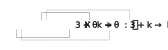
\includegraphics[width=80mm]{./img/Addition.png}
		\captionof{figure}{\textls[-50]{\mono{Bob's addition algorithm}}}
		\label{fig:addition}
	\end{minipage}	
	\vspace{4mm}
	
	In decimal representation, this is similar to 12 + 34 {\rightarrow} 1 : 2 + 3 : 4 {\rightarrow}  1 + 3 : 2 + 4 {\rightarrow} 4 : 6 {\rightarrow} 46. Bob is ecastatic! But he soon finds that in some cases, the sum of the individual digits is made up of two digits, whereas his primitive algorithm expects a single digit output. For example, consider the addition {\one\,\five} + {\two\,\six\,} {\rightarrow} {\one} + {\two} : {\five} + {\six\;\,}{\rightarrow} {\three} : {\one\,\four} {\rightarrow} {{?}}. It appears that Bob is stuck, or is he? Bob makes a quick observation that he just needs to split the pair {\one\,\four} on the right again, keep the relevant second digit {\four} and add the first digit {\one} to {\three}, such that 
	\vspace{4mm}
	\begin{center}
	{\one\,\five} + {\two\,\six\,} {\rightarrow} {\one} + {\two} : {\five} + {\six\;\,}{\rightarrow} {\three} : {\one\,\four} {\rightarrow} {\three} + {\one} : {\four} {\rightarrow} {\four\,\four}. 
	\end{center}
	\vspace{4mm}
	In decimal representation, this is similar to 15 + 26 {\rightarrow} 1 + 2 : 5 + 6 {\rightarrow} 3 : 11 {\rightarrow} 3 + 1 : 1 {\rightarrow} 4 : 1 {\rightarrow} 41. What we have described here is the method of addition by 'carrying' which we have all been taught in primary schools when we were kids, and it can be extended to add numbers with arbitrarily large digits. For example, 
	\vspace{4mm}
	\begin{center}
	{\seven\,\five} + {\two\,\six\,} {\rightarrow} {\seven} + {\two} : {\five} + {\six\;\,}{\rightarrow} {\one\,\three} : {\one\,\four} {\rightarrow} {\one\,\three} + {\one} : {\four} {\rightarrow} {\one\,\four} : {\four} {\rightarrow} {\one\,\four\,\four}, and
	\end{center}
	\vspace{4mm}
	In decimal representation, this is similar to 67 + 56 {\rightarrow} 6 + 5 : 7 + 6 {\rightarrow} 11 : 13 {\rightarrow} 11 + 1 : 3 {\rightarrow} 12 : 3 {\rightarrow} 123. The end of algorithm is determined by the : operator, i.e. when it has a single or pair to the left, at which point its function ends. In other words, the : operator always starts with a pair and ends with a single or pair to the left. For example,
	\vspace{4mm}
	\begin{center}
	{\one\,\seven\,\five} + {\three\,\two\,\six\,} {\rightarrow} {\four} : {\one\,\three} : {\one\,\four} {\rightarrow} {\four} : {\one\,\three} + {\one} : {\four} {\rightarrow} {\four} + {\one} : {\four} : {\four} {\rightarrow} {\five\,\four\,\four}.
	\end{center}
	\vspace{4mm}
	Once Bob discovers addition, it is only a matter of time before he realises that it is a {\mbold{commutative}}, symmteric and order-agnostic operation, i.e. {\one} + {\three} {\asserts} {\three} + {\one}. The symmetric natures simply follows from the fact that the total count after adding Bob and Alice's stones is the same whether you start by putting Alice's stones first on the lookup table or Bob's. This realisation quickly extended to {\mbold{associativity}} of addition, i.e. {\one} + {\three} + {\six\;\,}{\asserts} ({\one} + {\three}) + {\six\,} = {\one} + ({\three} + {\six\,}). It is only natural from here on for Bob to discover {\mbold{subtraction}} ({\three} - {\one} {\asserts} 3 - 1 = 2), which is simply the {\mbold{inverse}} of addition in the sense that it undos the effects of addition. However, Bob notes that it is anti-commutative, non-associative, asymmetric, order-dependent and it is in fact undefined when the order is reversed, i.e. {\one} - {\three}. This is because Bob has no concept of negative integers (he is restricted to natural numbers) and it makes no intuitive sense for him to subtract/remove a larger count of stones from a smaller collection (e.g. {\one} - {\three} {\asserts} 1 - 3 = {{?}}).\linebreak\linebreak
	}}
	\textls[-50]{\mono{With his newly found obsession of counting, Bob soon starts to remember most of the basic additions without explicitly needing to perform the stone table lookup. However, adding countably many stone collections remained a challenge, e.g. ({\seven\,\five} + {\five\,\two} + {\seven\,\five} + {\seven\,\three} + {\two\,\four} + {\seven\,\five} + {\seven\,\five} + {\seven\,\five} + {\seven\,\five} + \cdot\cdot\cdot) = ?. While dealing with such lengthy evaluations, Bob notices that when there are several stone collections with the same count, his task is relatively quite easy e.g. {\seven\,\five} featuring {\six\;\,}(=\;6) times in the above example. For instance, ({\seven\,\five} + {\seven\,\five} + {\seven\,\five} + {\seven\,\five} + {\seven\,\five} + {\seven\,\five}) is easier to evaluate since Bob remembers what he gets when he adds {\seven} (and {\five}) repeatedly {\six\;\,}(=\;6) times; he has performed this operation thousands of times in the past. In addition, he starts writing long evaluations like ({\seven\,\five} + {\seven\,\five} + {\seven\,\five} + {\seven\,\five} + {\seven\,\five} + {\seven\,\five}) as {\seven\,\five} {\times} {\six}, introducing the notation {\times} for describing repetitions in order to shorten his notation. Using his memory of simpler multiplications, Bob is able to perform his 'carry over' addition faster and soon doesn't need to use the expanded notation for {\times} at all! He can simply denote:
	
	\vspace{4mm}
	\begin{center}
	({\seven\,\five} + {\seven\,\five} + \cdot\cdot\cdot\;\raisebox{0.2ex}{\footnotesize{{\six\,} times}}\;\cdot\cdot\cdot) {\asserts} {\seven\,\five} {\times} {\six\;\,}{\rightarrow} {\seven}:{\five} {\times} {\six\;\,}{\rightarrow} {\seven} {\times} {\six\,} : {\five} {\times} {\six\,},
	\end{center}
	\vspace{4mm}
	followed by,
	\vspace{4mm}
	\begin{center}
	{\seven} {\times} {\six\,} : {\five} {\times} {\six\;\,}{\rightarrow} {\six\,\seven} : {\three\,\four} {\rightarrow} {\five\,\seven} + {\three} : {\four} {\rightarrow} {\six\,\three}:{\four} {\rightarrow} {\six\,\three\,\four}.
	\end{center}
	\vspace{4mm}
	In decimal notation, the above example is equivalent to:
	\vspace{4mm}
	\begin{center}
	(75 + 75 + \cdot\cdot\cdot\;\raisebox{0.2ex}{\footnotesize{6 times}}\;\cdot\cdot\cdot) {\asserts} 75 {\times} 6 {\rightarrow} 7 : 5 {\times} 6 {\rightarrow} 7 {\times} 6 : 5 {\times} 6
	\end{center}
	\begin{center}
	{\rightarrow} 42 : 30 {\rightarrow} 42 + 3 : 0 {\rightarrow} 45 : 0 {\rightarrow} 450.
	\end{center}
	\vspace{4mm}
	}}
	\textls[-50]{\mono{Curious bob immediately tests the multiplication operation for commutativity and associativity and finds that both properties hold; this doesn't come as a surprise to bob since he has constructed the {\times} operation from series of {+} operations which are both atomically commutative as well as associative. With the ability to perform complex counting operations, Bob soon rises among the ranks of stone gatherers and starts his own business. Soon he employs hundreds of gatherers and becomes a wholesale stone supplier.\linebreak\linebreak 
	With rising business however, he finds himself spending a lot of time doing lengthy operations, even after using his 'carry over' algorithm and memorised tables. One day he gets an unprecedented total of {\five\,\seven\,\two} (=\;345 in decimal) stone gatherers, each collecting anywhere between {\one\,\two} (=\;9) and {\one\,\seven\,\one} (=\;99) stones. This presented him with a huge number of table lookups and evaluations. For instance, he noted that there were {\five\,\seven} (=\;60) people who brought {\one\,\three\,\seven} (=\;93) stones each. Without his '{\times}' notation, Bob would need to make a record of it in the form of ({\five\,\seven} + {\five\,\seven} + \cdot\cdot\cdot \raisebox{0.2ex}{\footnotesize{\;{\one\,\three\,\seven} times}}\;\cdot\cdot\cdot). However, Bob uses his clever trick and quickly makes the abbreviation {\five\,\seven} {\times} {\one\,\three\,\seven} (=\;60\,{\times}\,93).\linebreak\linebreak 
	While the notation saves the day somewhat, it doesn't make Bob's job much easier. Unlike the previous (easier) example of 75 {\times} 6 where Bob remembered the multiplication table of 6, in this case he doesn't know the multiplcative table of either {\five\,\seven} (=\;60) or {\one\,\three\,\seven} (=\;93). While worried at the start, Bob soon realises that in fact only needs the tables of smallest atomic labels since {\five\,\seven} {\times} {\one\,\three\,\seven} {\rightarrow} {\five} {\times} {\one\,\three\,\seven} : {\seven} {\times} {\one\,\three\,\seven}, where both the left and right side of : can be individually evaluated as {\one\,\three\,\seven} {\times} {\five} {\asserts} {\one} {\times} {\five} : {\three} {\times} {\five} : {\seven} {\times} {\five} and {\one\,\three\,\seven} {\times} {\seven} {\asserts} {\one} {\times} {\seven} : {\three} {\times} {\seven} : {\seven} {\times} {\five} respectively, such that

	\vspace{4mm}
	\begin{center}
	{\five\,\seven} {\times} {\one\,\three\,\seven} {\rightarrow} {\five} {\times} {\one\,\three\,\seven} : {\seven} {\times} {\one\,\three\,\seven} {\rightarrow} ({\one} {\times} {\five} : {\three} {\times} {\five} : {\seven} {\times} {\five}) : ({\one} {\times} {\seven} : {\three} {\times} {\seven} : {\seven} {\times} {\seven}) {\rightarrow} ({\five} : {\two\,\one} : {\four\,\seven}) : ({\seven} : {\two\,\seven} : {\six\,\seven}) {\rightarrow} ({\seven} : {\five} : {\seven}) : ({\one\,\three} : {\six\;\,}: {\seven}) {\rightarrow} {\seven\,\five\,\seven} : {\one\,\three\,\six\,\seven} {\rightarrow} {\seven\,\five\,\seven} + {\one\,\three\,\six\;\,}: {\seven} {\rightarrow} {\one\,\two\,\two\,\six\;\,}: {\seven} {\rightarrow} {\one\,\two\,\two\,\six\,\seven}
	\end{center}
	\vspace{4mm}
	 In decimal world, this is similar to 
	 \vspace{4mm}
	\begin{center}
	 62 {\times} 99 {\rightarrow} 6 {\times} 99 : 2 {\times} 99 {\rightarrow} (6 {\times} 9 : 6 {\times} 9) : (2 {\times} 9 : 2 {\times} 9) {\rightarrow} (54 : 54) : (18 : 18) {\rightarrow} (54 + 4 : 4) : (18 + 1 : 8) {\rightarrow} (59 : 4) : (19 : 8) {\rightarrow} 594 : 198 {\rightarrow} 594 + 19 : 8 {\rightarrow} 6138.
	\end{center}
	\vspace{4mm}
	Using shorthand notation '{\times}' and lookup of simple multiplications in his memory, Bob is now able to calculate arbitrarily large multiplications with arbitrarily large arguments (stone count {\times} individuals with said stone count). What we have (re)constructed here is the well-known Vedic or Chinese or Japanese multiplication; one can imagine why there are so many names for it since it arises very naturally in any base system and was likely discovered independently by each intelligent civilisation.\linebreak\linebreak  
	Considering that Bob discovered the inverse of addition, it is natural for him to wonder if an inverse operation exists for multiplication; he denotes this operation with {\div}. In a countable sense, Bob interprets that {\mbold{division}} is equivalent to distributing a collection of stones equally among some individuals, e.g. he denotes his intention of dividing {\seven\,\three} stones among {\six\;\,}people with {\seven\,\three} {\div} {\six}. Bob initially deduces that division only makes sense if his collection of stones is sufficiently large to divide among any given group of people, i.e. for {\six\;\,}people, he needs at least {\six\;\,}stones to be able to give a single stone to everyone. This situation is similar to subtraction where Bob wasn't able to subtract a bigger count from a smaller count; now he is unable divide a smaller count by a bigger count. He finds that similar to subtraction, division is anti-commutative, non-associative, asymmetric and order-dependent. Bob lastly defines a corollary of division, the {\mbold{modulo}} operation {\%}, which describes how many stones will remain after Bob has finished equally distributing as many as he possibly can among all group members, e.g. {\seven\,\three} {\%} {\six} = {\four}. 
	\linebreak\linebreak\linebreak
	}}
	\textbf{\Large\pbold{PRIME COLLECTIONS}}\linebreak\linebreak
	\textls[-50]{\mono{Bob's good days are yet again shortlived. One day, he is assigned the task of dividing the day's collection of {\one\,\seven\,\three} stones equally among {\six\;\,}people in a group. Bob quickly finds that he is unable to do so; in decimal terms he had been asked to divide 101 stones among 6 people equally. He further notices that for a given group of people, some collections cannot be equally distributed. He also notes that for any given collection of stones, he can distribute it equally to only certains groups. In other words, not all numbers are divisible by other smaller numbers! This property is somewhat more bizarre to interpret for Bob; subtraction never caused him trouble in the sense that he could always distribute any collection of stones among any group of people as long as he didn't need to be fair and equal. Division seems to create more constraints for Bob when the condition of equality is imposed among all members of the group. Some days later, Bob's friend Arya noted that he was unable to equally divide his collection of {\one\,\seven\,\three} among {\one\,\two} (=\;9) people. Bob finds it odd that neither he nor his friend could equally distribute their equivalent collections of {\one\,\seven\,\three} (=\;101) stones to distinctly different groups of people (with 6 and 9 members). Bob investigates more and finds that the collection of {\one\,\seven\,\three} stones is in fact impossible to distribute equally among members of any countable group\textsuperscript{\textcolor{blue}{2}}\blfootnote{\textls[-50]{\mono{\textsuperscript{2}{with the exception of distributing a single stone per person}}}}; we know these numbers as {\mbold{prime numbers}}. Bob and Arya's investigations reveal that these numbers continue to exist no matter how far you extend the natural numbers, and their distribution is base-agnostic and aperiodic. 
	}}
	\textls[-50]{\mono{
	\linebreak\linebreak
	}}\linebreak
	\textbf{\Large\pbold{FINDING ZERO THROUGH ARITHMETIC}}\linebreak\linebreak
	\textls[-50]{\mono{Let's fast-forward a little bit and re-discover zero, i.e. 0. In figure \ref{fig:stones}, Arya notices that the horizontal and vertical axis are not the same 'stone units' in length, i.e. horizontal axis is one ({\rightarrow} {\one} {\rightarrow} 1) stone unit longer than vertical axis. Arya also notices that there is no formal label for describing complete absence of stones. He thereby suggests Bob that he should:
	 
	 \vspace{2mm}
	 {\hspace{4mm}}{\mbold{a)}} add one more cell representing {\zero} ({\rightarrow} {\zero\zero} {\rightarrow} {\zero\zero\zero}\;\cdot\cdot\cdot) at the top of the first column, and, 
	 
	 \vspace{2mm}
	 {\hspace{4mm}}{\mbold{b)}} introduce labels of the form {\one\zero}, {\two\zero}, {\three\zero}\,\cdot\cdot\cdot\,{\seven\zero} such that the table's axis are equal in length. 
	 
	 \vspace{2mm}
	 Bob however is not convinced since, 
	 
	 \vspace{2mm}
	 {\hspace{4mm}}{\mbold{i)}} he probably doesn't think that the 'absence of stones' needs a label, and secondly, 
	 
	 \vspace{2mm}
	 {\hspace{4mm}}{\mbold{ii)}} his intuitive interpretation of {\one\,\one} following {\seven} (i.e. first stone in the first column of paired labels) doesn't work if {\one\zero} happens to follow {\seven}. 
	 
	 \vspace{2mm}
	 Bob resists the idea of {\zero} for the longest time; infact, the concept of zero originated much later than the basic airthmetic operations of addition (+), subtraction (-), multiplication ($\times$) and division ($\div$). This is not surprising since these operations do not need zero in their primal definitions. The presence of zero however makes complex combinations (aka 'functions') of (+, -, $\times$, $\div$) much easier to describe/evaluate despite being unintuitive. This eventually led to the acceptance of zero ({\rightarrow} {\zero} {\rightarrow} 0) at par with natural numbers about 18,000 years later. In essence, zero makes natural numbers complete or 'whole', thus leading to the term {\mbold{whole numbers}}. In our fictional present however, Bob finds zero too abstract and unintuitive, and doesn't include it in his number system. With time, Bob's number system finds utility in all aspects of life, and being able to count and do basic airthmetic using the 'stone table' lookup in figure \ref{fig:stones} (which later became abacus) becomes equivalent to a Doctorate in Advanced Mathematics. Bob soon realises that he can not only count and describe objects using his system but he can quantify the 'size' of an object (once he assigns one stone unit to a specific size for setting a formal standard). By interpreting the table in \ref{fig:stones} such that each cell now represents the 'size' of an object, Bob discovers the concept of length (units along a string or line), area (units on flat surfaces) and volume (units inside bulky objects). In his native number system, the definition of length is the same as counting stone units along a path, say for example {\seven} units. The definition of area (with side length {\seven}) in his system yields ({\seven} + {\seven\,\times\,\seven}) units and the volume can be counted in ({\seven} + {\seven\,\times\,\seven} + {\seven\,\times\,\seven\,\times\,\seven}) units.\linebreak\linebreak
	 There is no reason for Bob to stop at multiplication and he can go on to formulate even more complex operations. For instance, recall that Bob derived multiplication from the idea of repetitive 'self-additions'; in the same spirit, Bob can now repeat multiplications to derive {\mbold{exponential}} operation, e.g. {\five}\textsuperscript{\seven} = {\five\,\times\,\five\,\times\,\cdot\cdot\cdot\,\raisebox{0.0ex}{\footnotesize{\seven}}\,\cdot\cdot\cdot\,\times\,\five}. Bob is further surprised to note that exponential operation is anti-commutative, non-associative, asymmetric, order-dependent; this isn't the case for either addition or multiplication - both of which are commutative, associative, symmetric and order-agnostic. It appears as if higher-order operations\textsuperscript{\textcolor{blue}{3}}\blfootnote{\textls[-50]{\mono{\textsuperscript{3}{addition = 1-order; multiplication = 2-order; exponential = 3-order}}}} generated from self-operating on lower-order operations leads to unusual behaviour after a certain order (=\;2-order).\linebreak\linebreak
	}}
	\colorbox{Gray}{\hspace{1mm}\parbox{0.99\textwidth}{\vspace{1mm}\textls[-50]{\mono{Let's take a sanity break and talk in 'normal' mathematical language. Note that in order to count to higher and higher values (more digits), Bob needs keep extending the dimensions of his 'counting box'. The 'counting volume' required to count up to {\upalpha} digits is then written as a series sum ({\seven} + {\seven}\textsuperscript{\two} + {\seven}\textsuperscript{\robot{^^^^03b8}} + \cdot\cdot\cdot\;\,+ {\seven}\textsuperscript{{\upalpha}}). This is somewhat inconvenient. Due to the asymmetric-by-1 nature of Bob's natural number system, many identities tend to have unnecessarily complex forms. In a whole number system however, the counting volume for {\upalpha} digits is simply ({\seven}\textsuperscript{\upalpha}); this is equivalent to 10\textsuperscript{{\upalpha}} digits in the decimal system. This finally convinces Bob to accept {\zero} in his counting system, thereby formalising whole numbers as the default counting framework.\vspace{1mm}}}}}\linebreak\linebreak\linebreak\linebreak
	\linebreak
	\textbf{\Large\pbold{REFERENCES}}\linebreak\linebreak
		\textls[-50]{\mono{
			[1] Intuitive Interpretation of Non-Interactive Zero-Knowledge Cryptography\linebreak
		}}
\end{flushleft}
\begin{flushright}
	\textbf{\large\pbold{METADATA}}\linebreak\linebreak
	\textls[-50]{\mono{
		\mono{Github: }\tcbox{}\linebreak
		\mono{Contracts: }\tcbox{}\linebreak
		\mono{Source: }\tcbox{}\linebreak
		\mono{SHA-1 Checksum: }\tcbox{}\linebreak
		\mono{Date: }\tcbox{\mono{\today}}\linebreak
	}}
\end{flushright}
\end{document}
